% Options for packages loaded elsewhere
\PassOptionsToPackage{unicode}{hyperref}
\PassOptionsToPackage{hyphens}{url}
%
\documentclass[
]{book}
\usepackage{amsmath,amssymb}
\usepackage{lmodern}
\usepackage{ifxetex,ifluatex}
\ifnum 0\ifxetex 1\fi\ifluatex 1\fi=0 % if pdftex
  \usepackage[T1]{fontenc}
  \usepackage[utf8]{inputenc}
  \usepackage{textcomp} % provide euro and other symbols
\else % if luatex or xetex
  \usepackage{unicode-math}
  \defaultfontfeatures{Scale=MatchLowercase}
  \defaultfontfeatures[\rmfamily]{Ligatures=TeX,Scale=1}
\fi
% Use upquote if available, for straight quotes in verbatim environments
\IfFileExists{upquote.sty}{\usepackage{upquote}}{}
\IfFileExists{microtype.sty}{% use microtype if available
  \usepackage[]{microtype}
  \UseMicrotypeSet[protrusion]{basicmath} % disable protrusion for tt fonts
}{}
\makeatletter
\@ifundefined{KOMAClassName}{% if non-KOMA class
  \IfFileExists{parskip.sty}{%
    \usepackage{parskip}
  }{% else
    \setlength{\parindent}{0pt}
    \setlength{\parskip}{6pt plus 2pt minus 1pt}}
}{% if KOMA class
  \KOMAoptions{parskip=half}}
\makeatother
\usepackage{xcolor}
\IfFileExists{xurl.sty}{\usepackage{xurl}}{} % add URL line breaks if available
\IfFileExists{bookmark.sty}{\usepackage{bookmark}}{\usepackage{hyperref}}
\hypersetup{
  pdftitle={Introduction to Theoretical Ecology},
  pdfauthor={Instructor: Po-Ju Ke \textasciitilde\textasciitilde\textasciitilde\textasciitilde\textasciitilde{} Teaching Assistant: Gen-Chang Hsu},
  hidelinks,
  pdfcreator={LaTeX via pandoc}}
\urlstyle{same} % disable monospaced font for URLs
\usepackage{color}
\usepackage{fancyvrb}
\newcommand{\VerbBar}{|}
\newcommand{\VERB}{\Verb[commandchars=\\\{\}]}
\DefineVerbatimEnvironment{Highlighting}{Verbatim}{commandchars=\\\{\}}
% Add ',fontsize=\small' for more characters per line
\usepackage{framed}
\definecolor{shadecolor}{RGB}{248,248,248}
\newenvironment{Shaded}{\begin{snugshade}}{\end{snugshade}}
\newcommand{\AlertTok}[1]{\textcolor[rgb]{0.94,0.16,0.16}{#1}}
\newcommand{\AnnotationTok}[1]{\textcolor[rgb]{0.56,0.35,0.01}{\textbf{\textit{#1}}}}
\newcommand{\AttributeTok}[1]{\textcolor[rgb]{0.77,0.63,0.00}{#1}}
\newcommand{\BaseNTok}[1]{\textcolor[rgb]{0.00,0.00,0.81}{#1}}
\newcommand{\BuiltInTok}[1]{#1}
\newcommand{\CharTok}[1]{\textcolor[rgb]{0.31,0.60,0.02}{#1}}
\newcommand{\CommentTok}[1]{\textcolor[rgb]{0.56,0.35,0.01}{\textit{#1}}}
\newcommand{\CommentVarTok}[1]{\textcolor[rgb]{0.56,0.35,0.01}{\textbf{\textit{#1}}}}
\newcommand{\ConstantTok}[1]{\textcolor[rgb]{0.00,0.00,0.00}{#1}}
\newcommand{\ControlFlowTok}[1]{\textcolor[rgb]{0.13,0.29,0.53}{\textbf{#1}}}
\newcommand{\DataTypeTok}[1]{\textcolor[rgb]{0.13,0.29,0.53}{#1}}
\newcommand{\DecValTok}[1]{\textcolor[rgb]{0.00,0.00,0.81}{#1}}
\newcommand{\DocumentationTok}[1]{\textcolor[rgb]{0.56,0.35,0.01}{\textbf{\textit{#1}}}}
\newcommand{\ErrorTok}[1]{\textcolor[rgb]{0.64,0.00,0.00}{\textbf{#1}}}
\newcommand{\ExtensionTok}[1]{#1}
\newcommand{\FloatTok}[1]{\textcolor[rgb]{0.00,0.00,0.81}{#1}}
\newcommand{\FunctionTok}[1]{\textcolor[rgb]{0.00,0.00,0.00}{#1}}
\newcommand{\ImportTok}[1]{#1}
\newcommand{\InformationTok}[1]{\textcolor[rgb]{0.56,0.35,0.01}{\textbf{\textit{#1}}}}
\newcommand{\KeywordTok}[1]{\textcolor[rgb]{0.13,0.29,0.53}{\textbf{#1}}}
\newcommand{\NormalTok}[1]{#1}
\newcommand{\OperatorTok}[1]{\textcolor[rgb]{0.81,0.36,0.00}{\textbf{#1}}}
\newcommand{\OtherTok}[1]{\textcolor[rgb]{0.56,0.35,0.01}{#1}}
\newcommand{\PreprocessorTok}[1]{\textcolor[rgb]{0.56,0.35,0.01}{\textit{#1}}}
\newcommand{\RegionMarkerTok}[1]{#1}
\newcommand{\SpecialCharTok}[1]{\textcolor[rgb]{0.00,0.00,0.00}{#1}}
\newcommand{\SpecialStringTok}[1]{\textcolor[rgb]{0.31,0.60,0.02}{#1}}
\newcommand{\StringTok}[1]{\textcolor[rgb]{0.31,0.60,0.02}{#1}}
\newcommand{\VariableTok}[1]{\textcolor[rgb]{0.00,0.00,0.00}{#1}}
\newcommand{\VerbatimStringTok}[1]{\textcolor[rgb]{0.31,0.60,0.02}{#1}}
\newcommand{\WarningTok}[1]{\textcolor[rgb]{0.56,0.35,0.01}{\textbf{\textit{#1}}}}
\usepackage{longtable,booktabs,array}
\usepackage{calc} % for calculating minipage widths
% Correct order of tables after \paragraph or \subparagraph
\usepackage{etoolbox}
\makeatletter
\patchcmd\longtable{\par}{\if@noskipsec\mbox{}\fi\par}{}{}
\makeatother
% Allow footnotes in longtable head/foot
\IfFileExists{footnotehyper.sty}{\usepackage{footnotehyper}}{\usepackage{footnote}}
\makesavenoteenv{longtable}
\usepackage{graphicx}
\makeatletter
\def\maxwidth{\ifdim\Gin@nat@width>\linewidth\linewidth\else\Gin@nat@width\fi}
\def\maxheight{\ifdim\Gin@nat@height>\textheight\textheight\else\Gin@nat@height\fi}
\makeatother
% Scale images if necessary, so that they will not overflow the page
% margins by default, and it is still possible to overwrite the defaults
% using explicit options in \includegraphics[width, height, ...]{}
\setkeys{Gin}{width=\maxwidth,height=\maxheight,keepaspectratio}
% Set default figure placement to htbp
\makeatletter
\def\fps@figure{htbp}
\makeatother
\setlength{\emergencystretch}{3em} % prevent overfull lines
\providecommand{\tightlist}{%
  \setlength{\itemsep}{0pt}\setlength{\parskip}{0pt}}
\setcounter{secnumdepth}{5}
\usepackage{booktabs}
\usepackage{booktabs}
\usepackage{longtable}
\usepackage{array}
\usepackage{multirow}
\usepackage{wrapfig}
\usepackage{float}
\usepackage{colortbl}
\usepackage{pdflscape}
\usepackage{tabu}
\usepackage{threeparttable}
\usepackage{threeparttablex}
\usepackage[normalem]{ulem}
\usepackage{makecell}
\usepackage{xcolor}
\ifluatex
  \usepackage{selnolig}  % disable illegal ligatures
\fi
\usepackage[]{natbib}
\bibliographystyle{apalike}

\title{Introduction to Theoretical Ecology}
\author{Instructor: Po-Ju Ke \(~~~~~\) Teaching Assistant: Gen-Chang Hsu}
\date{2021 Fall at National Taiwan Univeristy}

\begin{document}
\maketitle

{
\setcounter{tocdepth}{1}
\tableofcontents
}
\hypertarget{course-description}{%
\chapter*{Course description}\label{course-description}}
\addcontentsline{toc}{chapter}{Course description}

see the contents on ceiba

\hypertarget{requirements}{%
\section*{Requirements}\label{requirements}}
\addcontentsline{toc}{section}{Requirements}

see the contents on ceiba

\hypertarget{objectives}{%
\section*{Objectives}\label{objectives}}
\addcontentsline{toc}{section}{Objectives}

see the contents on ceiba

\hypertarget{course-information}{%
\chapter*{Course information}\label{course-information}}
\addcontentsline{toc}{chapter}{Course information}

course schedule and location

grading policy

contact info

office hours

\hypertarget{syllabus}{%
\chapter*{Syllabus}\label{syllabus}}
\addcontentsline{toc}{chapter}{Syllabus}

see the contents on ceiba

\begingroup\fontsize{20}{22}\selectfont

\begin{tabu} to \linewidth {>{\centering}X>{\centering}X}
\hline
\textcolor{black}{\textbf{Sepal.Length}} & \textcolor{black}{\textbf{Sepal.Width}}\\
\hline
\textbf{5.1} & \vphantom{1} 3.5\\
\hline
\textbf{4.9} & 3.0\\
\hline
\textbf{4.7} & \vphantom{1} 3.2\\
\hline
\textbf{4.6} & 3.1\\
\hline
\textbf{5.0} & 3.6\\
\hline
\textbf{5.4} & \vphantom{1} 3.9\\
\hline
\textbf{4.6} & 3.4\\
\hline
\textbf{5.0} & \vphantom{1} 3.4\\
\hline
\textbf{4.4} & 2.9\\
\hline
\textbf{4.9} & \vphantom{1} 3.1\\
\hline
\textbf{5.4} & 3.7\\
\hline
\textbf{4.8} & \vphantom{1} 3.4\\
\hline
\textbf{4.8} & \vphantom{1} 3.0\\
\hline
\textbf{4.3} & 3.0\\
\hline
\textbf{5.8} & 4.0\\
\hline
\textbf{5.7} & 4.4\\
\hline
\textbf{5.4} & 3.9\\
\hline
\textbf{5.1} & 3.5\\
\hline
\textbf{5.7} & 3.8\\
\hline
\textbf{5.1} & \vphantom{2} 3.8\\
\hline
\textbf{5.4} & \vphantom{1} 3.4\\
\hline
\textbf{5.1} & 3.7\\
\hline
\textbf{4.6} & 3.6\\
\hline
\textbf{5.1} & 3.3\\
\hline
\textbf{4.8} & 3.4\\
\hline
\textbf{5.0} & 3.0\\
\hline
\textbf{5.0} & 3.4\\
\hline
\textbf{5.2} & 3.5\\
\hline
\textbf{5.2} & 3.4\\
\hline
\textbf{4.7} & 3.2\\
\hline
\textbf{4.8} & 3.1\\
\hline
\textbf{5.4} & 3.4\\
\hline
\textbf{5.2} & 4.1\\
\hline
\textbf{5.5} & 4.2\\
\hline
\textbf{4.9} & 3.1\\
\hline
\textbf{5.0} & 3.2\\
\hline
\textbf{5.5} & 3.5\\
\hline
\textbf{4.9} & 3.6\\
\hline
\textbf{4.4} & 3.0\\
\hline
\textbf{5.1} & 3.4\\
\hline
\textbf{5.0} & \vphantom{1} 3.5\\
\hline
\textbf{4.5} & 2.3\\
\hline
\textbf{4.4} & 3.2\\
\hline
\textbf{5.0} & 3.5\\
\hline
\textbf{5.1} & \vphantom{1} 3.8\\
\hline
\textbf{4.8} & 3.0\\
\hline
\textbf{5.1} & 3.8\\
\hline
\textbf{4.6} & 3.2\\
\hline
\textbf{5.3} & 3.7\\
\hline
\textbf{5.0} & 3.3\\
\hline
\textbf{7.0} & 3.2\\
\hline
\textbf{6.4} & \vphantom{1} 3.2\\
\hline
\textbf{6.9} & \vphantom{2} 3.1\\
\hline
\textbf{5.5} & 2.3\\
\hline
\textbf{6.5} & 2.8\\
\hline
\textbf{5.7} & \vphantom{1} 2.8\\
\hline
\textbf{6.3} & \vphantom{1} 3.3\\
\hline
\textbf{4.9} & 2.4\\
\hline
\textbf{6.6} & 2.9\\
\hline
\textbf{5.2} & 2.7\\
\hline
\textbf{5.0} & 2.0\\
\hline
\textbf{5.9} & \vphantom{1} 3.0\\
\hline
\textbf{6.0} & \vphantom{1} 2.2\\
\hline
\textbf{6.1} & 2.9\\
\hline
\textbf{5.6} & 2.9\\
\hline
\textbf{6.7} & \vphantom{2} 3.1\\
\hline
\textbf{5.6} & \vphantom{1} 3.0\\
\hline
\textbf{5.8} & \vphantom{3} 2.7\\
\hline
\textbf{6.2} & 2.2\\
\hline
\textbf{5.6} & 2.5\\
\hline
\textbf{5.9} & 3.2\\
\hline
\textbf{6.1} & \vphantom{1} 2.8\\
\hline
\textbf{6.3} & \vphantom{1} 2.5\\
\hline
\textbf{6.1} & 2.8\\
\hline
\textbf{6.4} & 2.9\\
\hline
\textbf{6.6} & 3.0\\
\hline
\textbf{6.8} & 2.8\\
\hline
\textbf{6.7} & \vphantom{1} 3.0\\
\hline
\textbf{6.0} & 2.9\\
\hline
\textbf{5.7} & 2.6\\
\hline
\textbf{5.5} & \vphantom{1} 2.4\\
\hline
\textbf{5.5} & 2.4\\
\hline
\textbf{5.8} & \vphantom{2} 2.7\\
\hline
\textbf{6.0} & 2.7\\
\hline
\textbf{5.4} & 3.0\\
\hline
\textbf{6.0} & 3.4\\
\hline
\textbf{6.7} & \vphantom{1} 3.1\\
\hline
\textbf{6.3} & 2.3\\
\hline
\textbf{5.6} & 3.0\\
\hline
\textbf{5.5} & 2.5\\
\hline
\textbf{5.5} & 2.6\\
\hline
\textbf{6.1} & \vphantom{1} 3.0\\
\hline
\textbf{5.8} & 2.6\\
\hline
\textbf{5.0} & 2.3\\
\hline
\textbf{5.6} & 2.7\\
\hline
\textbf{5.7} & 3.0\\
\hline
\textbf{5.7} & 2.9\\
\hline
\textbf{6.2} & 2.9\\
\hline
\textbf{5.1} & 2.5\\
\hline
\textbf{5.7} & 2.8\\
\hline
\textbf{6.3} & 3.3\\
\hline
\textbf{5.8} & \vphantom{1} 2.7\\
\hline
\textbf{7.1} & 3.0\\
\hline
\textbf{6.3} & 2.9\\
\hline
\textbf{6.5} & \vphantom{2} 3.0\\
\hline
\textbf{7.6} & 3.0\\
\hline
\textbf{4.9} & 2.5\\
\hline
\textbf{7.3} & 2.9\\
\hline
\textbf{6.7} & 2.5\\
\hline
\textbf{7.2} & 3.6\\
\hline
\textbf{6.5} & 3.2\\
\hline
\textbf{6.4} & 2.7\\
\hline
\textbf{6.8} & 3.0\\
\hline
\textbf{5.7} & 2.5\\
\hline
\textbf{5.8} & 2.8\\
\hline
\textbf{6.4} & 3.2\\
\hline
\textbf{6.5} & \vphantom{1} 3.0\\
\hline
\textbf{7.7} & 3.8\\
\hline
\textbf{7.7} & 2.6\\
\hline
\textbf{6.0} & 2.2\\
\hline
\textbf{6.9} & 3.2\\
\hline
\textbf{5.6} & 2.8\\
\hline
\textbf{7.7} & 2.8\\
\hline
\textbf{6.3} & 2.7\\
\hline
\textbf{6.7} & \vphantom{1} 3.3\\
\hline
\textbf{7.2} & 3.2\\
\hline
\textbf{6.2} & 2.8\\
\hline
\textbf{6.1} & 3.0\\
\hline
\textbf{6.4} & \vphantom{1} 2.8\\
\hline
\textbf{7.2} & 3.0\\
\hline
\textbf{7.4} & 2.8\\
\hline
\textbf{7.9} & 3.8\\
\hline
\textbf{6.4} & 2.8\\
\hline
\textbf{6.3} & 2.8\\
\hline
\textbf{6.1} & 2.6\\
\hline
\textbf{7.7} & 3.0\\
\hline
\textbf{6.3} & 3.4\\
\hline
\textbf{6.4} & 3.1\\
\hline
\textbf{6.0} & 3.0\\
\hline
\textbf{6.9} & \vphantom{1} 3.1\\
\hline
\textbf{6.7} & 3.1\\
\hline
\textbf{6.9} & 3.1\\
\hline
\textbf{5.8} & 2.7\\
\hline
\textbf{6.8} & 3.2\\
\hline
\textbf{6.7} & 3.3\\
\hline
\textbf{6.7} & 3.0\\
\hline
\textbf{6.3} & 2.5\\
\hline
\textbf{6.5} & 3.0\\
\hline
\textbf{6.2} & 3.4\\
\hline
\textbf{5.9} & 3.0\\
\hline
\end{tabu}
\endgroup{}

\hypertarget{week-1}{%
\chapter*{Week 1}\label{week-1}}
\addcontentsline{toc}{chapter}{Week 1}

Figure with label and caption

\begin{Shaded}
\begin{Highlighting}[]
\FunctionTok{par}\NormalTok{(}\AttributeTok{mar =} \FunctionTok{c}\NormalTok{(}\DecValTok{4}\NormalTok{, }\DecValTok{4}\NormalTok{, .}\DecValTok{1}\NormalTok{, .}\DecValTok{1}\NormalTok{))}
\FunctionTok{plot}\NormalTok{(pressure, }\AttributeTok{type =} \StringTok{\textquotesingle{}b\textquotesingle{}}\NormalTok{, }\AttributeTok{pch =} \DecValTok{19}\NormalTok{)}
\end{Highlighting}
\end{Shaded}

\begin{figure}

{\centering 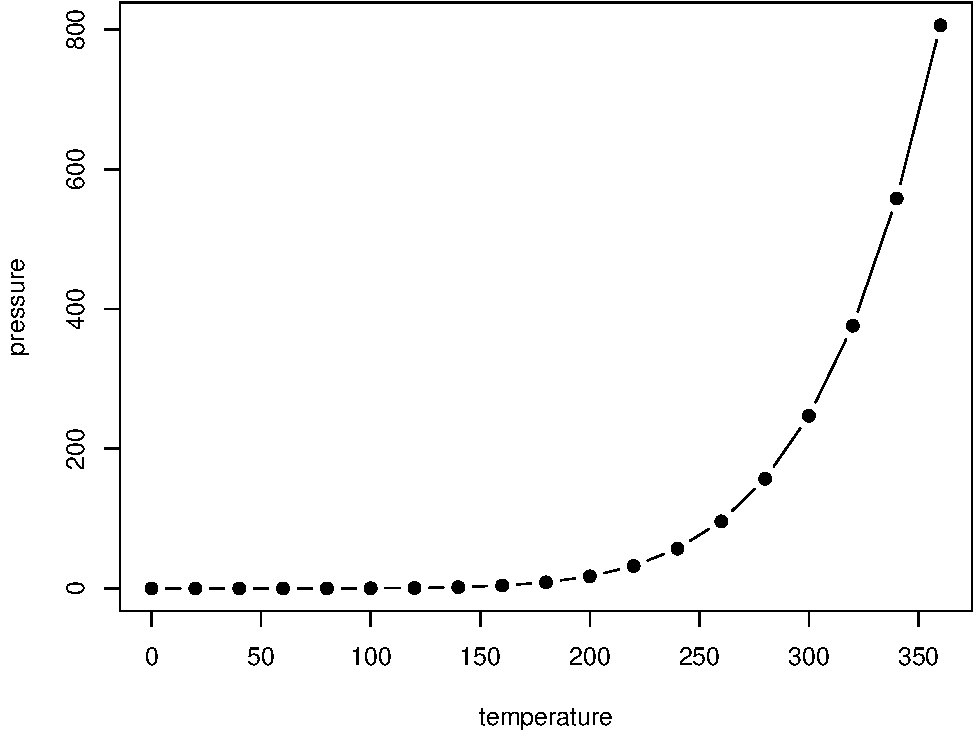
\includegraphics[width=0.8\linewidth]{01_Week_1_files/figure-latex/nice-fig-1} 

}

\caption{Here is a nice figure!}\label{fig:nice-fig}
\end{figure}

External image with label and caption

\begin{Shaded}
\begin{Highlighting}[]
\NormalTok{knitr}\SpecialCharTok{::}\FunctionTok{include\_graphics}\NormalTok{(}\StringTok{"knit{-}logo.png"}\NormalTok{)}
\end{Highlighting}
\end{Shaded}

\begin{figure}

{\centering 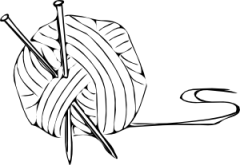
\includegraphics[width=0.8\linewidth]{knit-logo} 

}

\caption{Here is a nice figure!}\label{fig:nice-fig2}
\end{figure}

Table with label and caption

\begin{Shaded}
\begin{Highlighting}[]
\NormalTok{knitr}\SpecialCharTok{::}\FunctionTok{kable}\NormalTok{(}
  \FunctionTok{head}\NormalTok{(iris, }\DecValTok{20}\NormalTok{), }\AttributeTok{caption =} \StringTok{\textquotesingle{}Here is a nice table!\textquotesingle{}}\NormalTok{,}
  \AttributeTok{booktabs =} \ConstantTok{TRUE}
\NormalTok{)}
\end{Highlighting}
\end{Shaded}

\begin{table}

\caption{\label{tab:nice-tab}Here is a nice table!}
\centering
\begin{tabular}[t]{rrrrl}
\toprule
Sepal.Length & Sepal.Width & Petal.Length & Petal.Width & Species\\
\midrule
5.1 & 3.5 & 1.4 & 0.2 & setosa\\
4.9 & 3.0 & 1.4 & 0.2 & setosa\\
4.7 & 3.2 & 1.3 & 0.2 & setosa\\
4.6 & 3.1 & 1.5 & 0.2 & setosa\\
5.0 & 3.6 & 1.4 & 0.2 & setosa\\
\addlinespace
5.4 & 3.9 & 1.7 & 0.4 & setosa\\
4.6 & 3.4 & 1.4 & 0.3 & setosa\\
5.0 & 3.4 & 1.5 & 0.2 & setosa\\
4.4 & 2.9 & 1.4 & 0.2 & setosa\\
4.9 & 3.1 & 1.5 & 0.1 & setosa\\
\addlinespace
5.4 & 3.7 & 1.5 & 0.2 & setosa\\
4.8 & 3.4 & 1.6 & 0.2 & setosa\\
4.8 & 3.0 & 1.4 & 0.1 & setosa\\
4.3 & 3.0 & 1.1 & 0.1 & setosa\\
5.8 & 4.0 & 1.2 & 0.2 & setosa\\
\addlinespace
5.7 & 4.4 & 1.5 & 0.4 & setosa\\
5.4 & 3.9 & 1.3 & 0.4 & setosa\\
5.1 & 3.5 & 1.4 & 0.3 & setosa\\
5.7 & 3.8 & 1.7 & 0.3 & setosa\\
5.1 & 3.8 & 1.5 & 0.3 & setosa\\
\bottomrule
\end{tabular}
\end{table}

\protect\hyperlink{abcd}{Internal Link to anchor}

\hypertarget{equations}{%
\section*{Equations}\label{equations}}
\addcontentsline{toc}{section}{Equations}

\(f(k) = {n \choose k} p^{k} (1-p)^{n-k}\)

\[f(k) = {n \choose k} p^{k} (1-p)^{n-k}\]

\[\begin{vmatrix}a & b\\
c & d
\end{vmatrix}=ad-bc\]

\begin{equation} 
  f\left(k\right) = \binom{n}{k} p^k\left(1-p\right)^{n-k}
  \label{eq:binom}
\end{equation}

\begin{equation*} 
\frac{d}{dx}\left( \int_{a}^{x} f(u)\,du\right)=f(x)
\end{equation*}

Text references



\begin{Shaded}
\begin{Highlighting}[]
\FunctionTok{plot}\NormalTok{(cars)  }\CommentTok{\# a scatterplot}
\end{Highlighting}
\end{Shaded}

\begin{figure}
\centering
\includegraphics{01_Week_1_files/figure-latex/foo-1.pdf}
\caption{\label{fig:foo}A scatterplot of the data \texttt{cars} using \textbf{base} R graphics.}
\end{figure}

see this!!!

\hypertarget{week-2}{%
\chapter*{Week 2}\label{week-2}}
\addcontentsline{toc}{chapter}{Week 2}

\begin{Shaded}
\begin{Highlighting}[]
\FunctionTok{plot}\NormalTok{(cars)  }\CommentTok{\# a scatterplot}
\end{Highlighting}
\end{Shaded}

\begin{figure}
\centering
\includegraphics{02_Week_2_files/figure-latex/foo-1.pdf}
\caption{\label{fig:foo}A scatterplot of the data \texttt{cars} using \textbf{base} R graphics.}
\end{figure}

\protect\hyperlink{course-information}{Course information}

\protect\hyperlink{course-information}{non-English books}

\protect\hyperlink{equations}{non-English books2}

Figure \ref{fig:nice-fig}

Figure \ref{fig:nice-fig2}

Figure \ref{fig:foo}

Equation \eqref{eq:binom}

\hypertarget{cross-reference}{%
\section*{Cross-reference}\label{cross-reference}}
\addcontentsline{toc}{section}{Cross-reference}

Reference a figure by its code chunk label with the \texttt{fig:} prefix, e.g., see Figure \ref{fig:nice-fig}. Similarly, you can reference tables generated from \texttt{knitr::kable()}, e.g., see Table \ref{tab:nice-tab}.

see \citet{R-base} for details

also \citet{R-bookdown} for details

  \bibliography{book.bib,packages.bib}

\end{document}
